% groove cheat sheet: two landscape A4 pages.  Build: make cheatsheet
% Every number here comes from lib/groove_ctl.h, lib/groove_seq.h,
% lib/groove_synth.h, lib/groove_drums.h and objects/kit_bb/CREDITS.md.
\documentclass{article}
\usepackage[a4paper,landscape,margin=6mm]{geometry}
\usepackage[T1]{fontenc}
\usepackage{lmodern}
\usepackage[default]{sourcesanspro}
\usepackage{amssymb}
\usepackage{tikz}
\usepackage[most]{tcolorbox}
\usepackage{array}
\usepackage{tabularx}
\pagestyle{empty}
\setlength{\parindent}{0pt}

\definecolor{ink}{RGB}{30,30,30}
\definecolor{snd}{RGB}{20,20,20}       % SYNTH page
\definecolor{gvc}{RGB}{30,90,170}      % GROOVE page
\definecolor{drc}{RGB}{200,90,20}      % drums
\definecolor{chc}{RGB}{120,60,170}     % chords / synth
\definecolor{fltc}{RGB}{215,60,50}     % filter
\definecolor{trc}{RGB}{0,130,120}      % transport / looper
\definecolor{padc}{RGB}{120,170,230}
\definecolor{freec}{RGB}{170,170,170}

\newcommand{\GV}[1]{\textcolor{gvc}{#1}}
\newcommand{\DR}[1]{\textcolor{drc}{#1}}
\newcommand{\CH}[1]{\textcolor{chc}{#1}}
\newcommand{\TR}[1]{\textcolor{trc}{#1}}
\newcommand{\cc}[1]{\textcolor{black!45}{\fontsize{4.6}{5}\selectfont #1}}
\newcommand{\st}[1]{\\[-0.5mm]{\fontsize{4.4}{5}\selectfont\color{black!50}#1}}

\newcommand{\knob}[3]{%
  \draw[fill=black!8, draw=black!60, line width=0.4pt] (#1,62) circle (3.6);
  \draw[black!60, line width=0.5pt] (#1,62) -- ++(110:3.1);
  \node[font=\fontsize{5.6}{6.2}\selectfont\bfseries, text=snd, align=center] at (#1,69.4) {#2};
  \node[font=\fontsize{5.6}{6.2}\selectfont, text=gvc, align=center] at (#1,54.4) {#3};}
\newcommand{\pad}[3]{%
  \draw[rounded corners=0.8mm, fill=padc!35!white, draw=padc!80!black, line width=0.4pt]
    (36+#1*13.2, 21+#2*13.2) rectangle ++(12,12);
  \node[font=\fontsize{5.2}{5.8}\selectfont, text=ink, align=center, text width=11.5mm]
    at (36+#1*13.2+6, 21+#2*13.2+6) {#3};}
\newcommand{\fader}[3]{%
  \draw[fill=black!12, draw=black!50] (#1-0.7,26) rectangle (#1+0.7,52);
  \draw[fill=#3!60!white, draw=#3!70!black, rounded corners=0.4mm] (#1-2.6,36) rectangle (#1+2.6,40);
  \node[font=\fontsize{5.2}{5.8}\selectfont\bfseries, text=#3!70!black, align=center] at (#1,56) {#2};}
\newcommand{\btn}[5]{%
  \draw[rounded corners=0.6mm, fill=#4!25!white, draw=#4!70!black, line width=0.4pt]
    (#1-#5/2,#2-2.6) rectangle (#1+#5/2,#2+2.6);
  \node[font=\fontsize{4.9}{5.4}\selectfont, text=ink, align=center] at (#1,#2) {#3};}

\tcbset{card/.style={enhanced, colback=white, colframe=black!70, boxrule=0.5pt, arc=1.5mm,
    left=1.6mm, right=1.6mm, top=1.1mm, bottom=1.1mm, toptitle=0.6mm, bottomtitle=0.6mm,
    fonttitle=\bfseries\fontsize{8.6}{10}\selectfont, coltitle=white, colbacktitle=black!75,
    fontupper=\fontsize{7.1}{8.5}\selectfont, before skip=0mm, after skip=1.8mm}}
\newtcolorbox{card}[1]{card, title={#1}}
\newcolumntype{L}{>{\raggedright\arraybackslash}X}

\begin{document}

{\fontsize{16}{18}\selectfont\bfseries groove}\hspace{3mm}%
{\fontsize{9.5}{11}\selectfont Axoloti Core + Launchkey 49 MK3 (standalone mode) \textperiodcentered{}
real-time looper: sampled drums + 4-voice chords \textperiodcentered{} \texttt{patches/groove/groove\_v1.axp}}\hfill
{\fontsize{7}{8}\selectfont\color{black!55} v1.0 \textperiodcentered{} 2026-11-11 \textperiodcentered{} page 1 of 2}

\vspace{1.5mm}
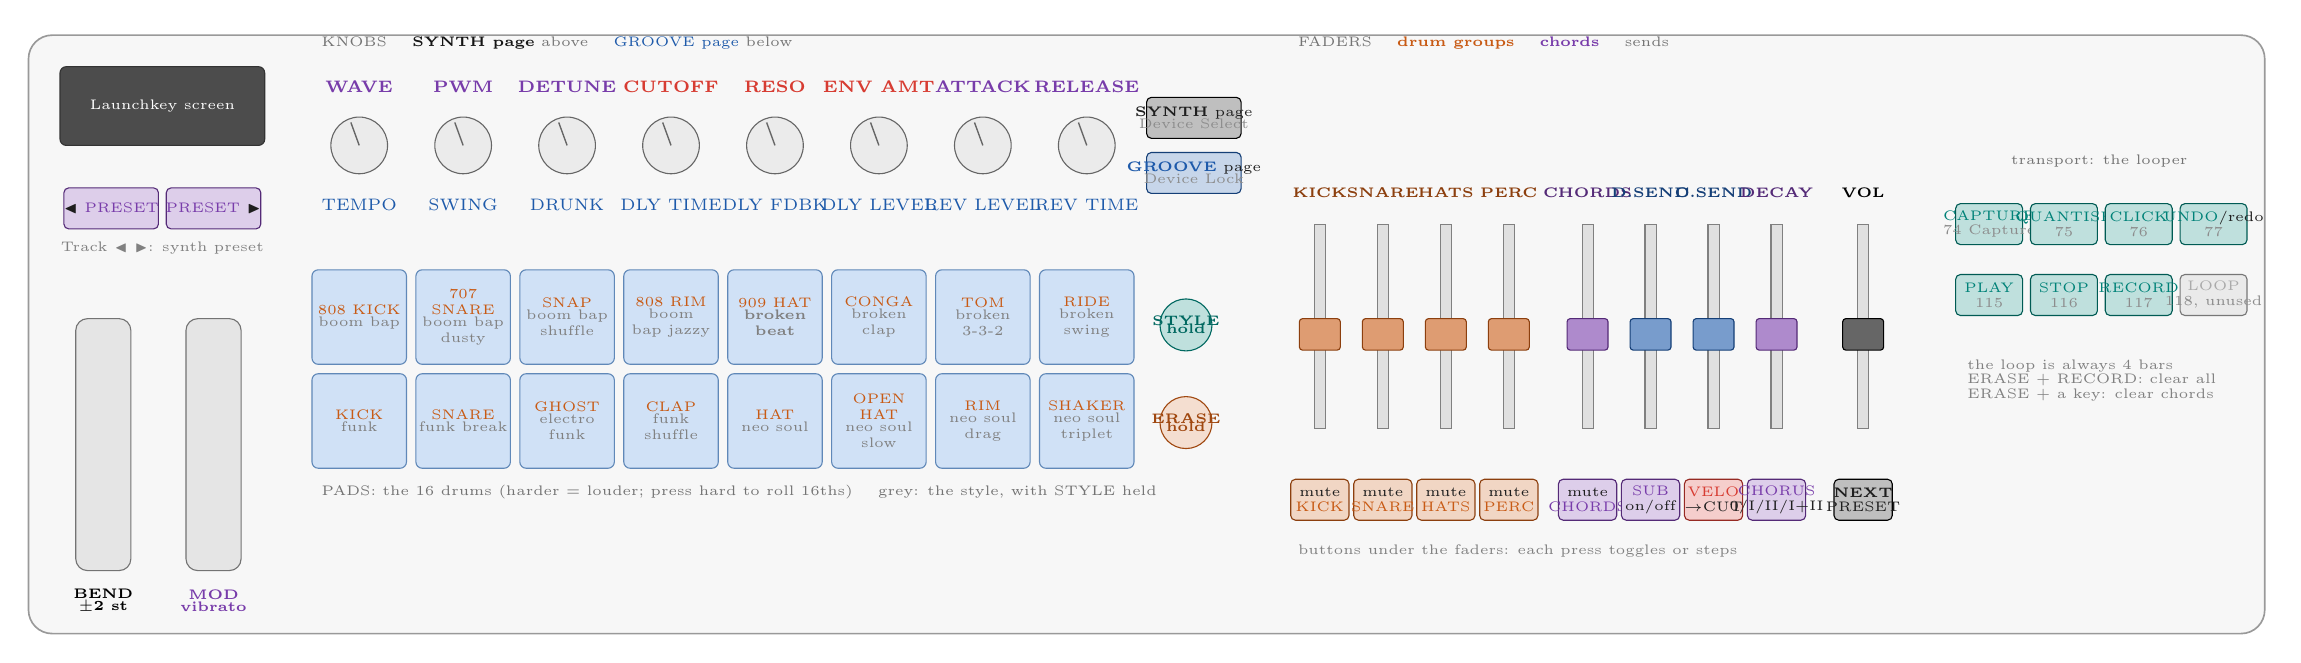
\begin{tikzpicture}[x=1mm,y=1mm]
  \draw[rounded corners=3mm, fill=black!3, draw=black!40, line width=0.6pt] (0,0) rectangle (284,76);

  \draw[fill=black!70, draw=black!80, rounded corners=0.8mm] (4,62) rectangle (30,72);
  \node[font=\fontsize{5}{6}\selectfont, text=white] at (17,67) {Launchkey screen};
  \btn{10.5}{54}{\(\blacktriangleleft\) \CH{PRESET}}{chc}{12}
  \btn{23.5}{54}{\CH{PRESET} \(\blacktriangleright\)}{chc}{12}
  \node[font=\fontsize{4.6}{5}\selectfont, text=black!50] at (17,49) {Track \(\blacktriangleleft\) \(\blacktriangleright\): synth preset};
  \draw[rounded corners=1.5mm, fill=black!10, draw=black!55] (6,8) rectangle (13,40);
  \draw[rounded corners=1.5mm, fill=black!10, draw=black!55] (20,8) rectangle (27,40);
  \node[font=\fontsize{5.4}{6}\selectfont\bfseries, align=center] at (9.5,4.2) {BEND\\[-0.6mm]\(\pm\)2 st};
  \node[font=\fontsize{5.4}{6}\selectfont\bfseries, align=center, text=chc] at (23.5,4.2) {MOD\\[-0.6mm]vibrato};

  \node[font=\fontsize{5}{6}\selectfont, text=black!55, anchor=west] at (36,75) {KNOBS \quad
     \textbf{\textcolor{snd}{SYNTH page}} above \quad \GV{GROOVE page} below};
  \knob{42}{\CH{WAVE}}{\GV{TEMPO}}
  \knob{55.2}{\CH{PWM}}{\GV{SWING}}
  \knob{68.4}{\CH{DETUNE}}{\GV{DRUNK}}
  \knob{81.6}{\textcolor{fltc}{CUTOFF}}{\GV{DLY TIME}}
  \knob{94.8}{\textcolor{fltc}{RESO}}{\GV{DLY FDBK}}
  \knob{108}{\textcolor{fltc}{ENV AMT}}{\GV{DLY LEVEL}}
  \knob{121.2}{\CH{ATTACK}}{\GV{REV LEVEL}}
  \knob{134.4}{\CH{RELEASE}}{\GV{REV TIME}}
  \btn{148}{65.5}{\textbf{SYNTH} page\\[-0.4mm]\cc{Device Select}}{black}{12}
  \btn{148}{58.5}{\textbf{\GV{GROOVE}} page\\[-0.4mm]\cc{Device Lock}}{gvc}{12}

  % pads: kit pad (style while the upper round button is held)
  \pad{0}{1}{\DR{808 KICK}\st{boom bap}}  \pad{1}{1}{\DR{707 SNARE}\st{boom bap dusty}}  \pad{2}{1}{\DR{SNAP}\st{boom bap shuffle}}
  \pad{3}{1}{\DR{808 RIM}\st{boom bap jazzy}} \pad{4}{1}{\DR{909 HAT}\st{\textbf{broken beat}}} \pad{5}{1}{\DR{CONGA}\st{broken clap}}
  \pad{6}{1}{\DR{TOM}\st{broken 3-3-2}} \pad{7}{1}{\DR{RIDE}\st{broken swing}}
  \pad{0}{0}{\DR{KICK}\st{funk}} \pad{1}{0}{\DR{SNARE}\st{funk break}} \pad{2}{0}{\DR{GHOST}\st{electro funk}}
  \pad{3}{0}{\DR{CLAP}\st{funk shuffle}} \pad{4}{0}{\DR{HAT}\st{neo soul}} \pad{5}{0}{\DR{OPEN HAT}\st{neo soul slow}}
  \pad{6}{0}{\DR{RIM}\st{neo soul drag}} \pad{7}{0}{\DR{SHAKER}\st{neo soul triplet}}
  \node[font=\fontsize{5}{6}\selectfont, text=black!55, anchor=west] at (36,18) {PADS: the 16 drums (harder = louder; press hard to roll 16ths) \quad grey: the style, with STYLE held};
  \draw[fill=trc!25!white, draw=trc!80!black] (147,39.2) circle (3.3);
  \draw[fill=drc!20!white, draw=drc!80!black] (147,26.8) circle (3.3);
  \node[font=\fontsize{4.6}{5}\selectfont\bfseries, align=center, text=trc!80!black] at (147,39.2) {STYLE\\[-0.8mm]hold};
  \node[font=\fontsize{4.6}{5}\selectfont\bfseries, align=center, text=drc!80!black] at (147,26.8) {ERASE\\[-0.8mm]hold};

  \node[font=\fontsize{5}{6}\selectfont, text=black!55, anchor=west] at (160,75) {FADERS \quad
     \DR{\textbf{drum groups}} \quad \CH{\textbf{chords}} \quad sends};
  \fader{164}{KICK}{drc} \fader{172}{SNARE}{drc} \fader{180}{HATS}{drc} \fader{188}{PERC}{drc}
  \fader{198}{CHORDS}{chc} \fader{206}{D.SEND}{gvc} \fader{214}{C.SEND}{gvc} \fader{222}{DECAY}{chc}
  \fader{233}{VOL}{black}
  \btn{164}{17}{mute\\\DR{KICK}}{drc}{7.4}
  \btn{172}{17}{mute\\\DR{SNARE}}{drc}{7.4}
  \btn{180}{17}{mute\\\DR{HATS}}{drc}{7.4}
  \btn{188}{17}{mute\\\DR{PERC}}{drc}{7.4}
  \btn{198}{17}{mute\\\CH{CHORDS}}{chc}{7.4}
  \btn{206}{17}{\CH{SUB}\\on/off}{chc}{7.4}
  \btn{214}{17}{\textcolor{fltc}{VELO}\\\(\to\)CUT}{fltc}{7.4}
  \btn{222}{17}{\CH{CHORUS}\\0/I/II/I+II}{chc}{7.4}
  \btn{233}{17}{\textbf{NEXT}\\PRESET}{black}{7.4}
  \node[font=\fontsize{4.6}{5}\selectfont, text=black!50, anchor=west] at (160,10.5) {buttons under the faders: each press toggles or steps};

  \node[font=\fontsize{5}{6}\selectfont, text=black!55] at (263,60) {transport: the looper};
  \btn{249}{52}{\TR{CAPTURE}\\\cc{74 Capture}}{trc}{8.5}
  \btn{258.5}{52}{\TR{QUANTISE}\\\cc{75}}{trc}{8.5}
  \btn{268}{52}{\TR{CLICK}\\\cc{76}}{trc}{8.5}
  \btn{277.5}{52}{\TR{UNDO}/redo\\\cc{77}}{trc}{8.5}
  \btn{249}{43}{\TR{PLAY}\\\cc{115}}{trc}{8.5}
  \btn{258.5}{43}{\TR{STOP}\\\cc{116}}{trc}{8.5}
  \btn{268}{43}{\TR{RECORD}\\\cc{117}}{trc}{8.5}
  \btn{277.5}{43}{\textcolor{freec}{LOOP}\\\cc{118, unused}}{freec}{8.5}
  \node[font=\fontsize{4.6}{5.2}\selectfont, text=black!50, align=left, anchor=north west] at (245,36)
     {the loop is always 4 bars\\ERASE + RECORD: clear all\\ERASE + a key: clear chords};
\end{tikzpicture}

\vspace{1.2mm}
\begin{minipage}[t]{72mm}\vspace{0pt}
\begin{card}{The looper}
\textbf{Start}: hold \TR{STYLE} and tap a pad: drums written in that style for the whole loop
and its tempo, swing and drunk (bars 1--3 the style, bar 4 a variation). \TR{PLAY}. Tap the same pad again (STYLE held) for a new variation.\\[0.4mm]
\textbf{Record}: \TR{RECORD} records what you play, on top of the loop (from stopped it starts the loop
at bar 1). Press again to stop recording; the loop plays on.\\[0.4mm]
\textbf{Drums} you play land on the 16th grid when \TR{QUANTISE} is on (power-on), with the swing.
\textbf{Chords} are kept exactly as played, held notes and all; the sustain pedal holds them.\\[0.4mm]
\textbf{Capture}: play over the running loop without recording; if you like it, \TR{CAPTURE} puts the last
loop-length you played into the loop.\\[0.4mm]
\textbf{Undo} takes back the last pass (recording, style, erase, clear); pressed again it redoes.\\[0.4mm]
\textbf{Erase}: hold \DR{ERASE} and tap a pad: that drum's hits leave the loop.
\end{card}
\end{minipage}\hfill
\begin{minipage}[t]{70mm}\vspace{0pt}
\begin{card}{Groove}
\GV{\textbf{TEMPO}} 70 -- 140 BPM. \GV{\textbf{SWING}} as on an MPC: the first 16th of each pair takes
50 -- 75\,\% of it. \GV{\textbf{DRUNK}}: grid hits land late by a random amount, new every bar, up to a third
of a 16th; never the kicks. A style sets all three (page 2); a variation keeps them. After a style,
a knob takes over when turned through its value.
\end{card}
\begin{card}{Chords: the synth}
4 voices (a 5th note takes the oldest). Two oscillators: \CH{WAVE} saw \(\to\) pulse, \CH{PWM} its
width wobble, \CH{DETUNE} brings in the second oscillator then detunes it (0 -- 25 cents);
\CH{SUB} an octave down. 24 dB/oct low-pass: \textcolor{fltc}{CUTOFF}, \textcolor{fltc}{RESO}, \textcolor{fltc}{ENV AMT}
(0 -- 6 octaves of filter envelope, by velocity with VELO\(\to\)CUT). \CH{ATTACK}, \CH{DECAY} (fader 8),
\CH{RELEASE} for both envelopes; the preset sets the sustains. \CH{CHORUS} as the Juno's.
\end{card}
\end{minipage}\hfill
\begin{minipage}[t]{68mm}\vspace{0pt}
\begin{card}{Mix and effects}
Faders 1--4: drum groups (\DR{KICK}: kicks; \DR{SNARE}: snares, ghost, clap, snap;
\DR{HATS}: hats, ride; \DR{PERC}: rims, shaker, conga, tom). Fader 5 the chords. Buttons 1--5 mute them
(the loop goes on). Faders 6, 7: how much of the drums and of the chords goes to the effects:
a delay in beats (\GV{DLY TIME}: 1/16, 1/8, dotted 1/8, 1/4, dotted 1/4, 1/2) into the Elements reverb.
\end{card}
\begin{card}{Rolls}
Press a pad hard (past 3/4 of its pressure) while the loop runs: it repeats every 16th at the
pressure's velocity, swung, and is recorded when recording.
\end{card}
\end{minipage}\hfill
\begin{minipage}[t]{63mm}\vspace{0pt}
\begin{card}{Its own SD card}
grains and groove each live on their own card; freak in flash when there is none.
\textbf{Install}: open \texttt{groove\_v1.axp}, \emph{Upload to SD Card as Startup}: it also copies the kit to
\texttt{/kit}. \textbf{Your own kit}: \texttt{/kit/NN\_name.wav}, NN = 01 -- 16 is the pad (any WAV:
16/24/32-bit, float, any rate, stereo mixed to mono). Without files the pads play built-in stand-ins.
\end{card}
\begin{card}{Signal path}
pads, loop \(\to\) 16 drum voices; keys, loop \(\to\) 4 synth voices \(\to\) chorus \(\to\) mix
(sends \(\to\) delay \(\to\) reverb) \(\to\) VOL. The loop holds up to 768 events, 4 bars.
\end{card}
\end{minipage}

%======================================================================
\newpage
{\fontsize{16}{18}\selectfont\bfseries groove}\hspace{3mm}%
{\fontsize{9.5}{11}\selectfont styles, kit, presets, dial values, troubleshooting}\hfill
{\fontsize{7}{8}\selectfont\color{black!55} v1.0 \textperiodcentered{} page 2 of 2}

\vspace{1.5mm}
\begin{minipage}[t]{150mm}\vspace{0pt}
\begin{card}{The 16 drum styles: hold STYLE + pad \quad\textmd{\fontsize{6.5}{7}\selectfont (each sets tempo, swing as MPC \%, drunk 0 -- 1; bars: its phrase)}}
\fontsize{7}{8.4}\selectfont
\setlength{\tabcolsep}{1.9pt}
\begin{tabular}[t]{@{}r l r r r c l@{}}
pad & style & BPM & swing & drunk & bars & sounds \\ \hline
1 & funk & 100 & 52 & 0 & 1 & 909 hats, ghost notes \\
2 & funk break & 104 & 50 & 0 & 2 & 707 snare, conga \\
3 & electro funk & 112 & 50 & 0 & 1 & 808 kick, clap \\
4 & funk shuffle & 96 & 62 & 0.08 & 1 & half time, ghosts \\
5 & neo soul & 84 & 62 & 0.50 & 2 & 808 kick, rim, shaker \\
6 & neo soul slow & 76 & 64 & 0.39 & 1 & snap + clap \\
7 & neo soul drag & 88 & 60 & 0.71 & 1 & snare, hats late \\
8 & neo soul triplet & 80 & 66 & 0.31 & 1 & ride, rim, conga \\
\end{tabular}\hfill
\begin{tabular}[t]{@{}r l r r r c l@{}}
pad & style & BPM & swing & drunk & bars & sounds \\ \hline
9 & boom bap & 90 & 60 & 0.08 & 2 & 909 kick, snare \\
10 & boom bap dusty & 86 & 62 & 0.16 & 1 & 808 kick, rim \\
11 & boom bap shuffle & 92 & 64 & 0 & 1 & clap + snare \\
12 & boom bap jazzy & 88 & 62 & 0.24 & 2 & ride, 707 snare \\
13 & \textbf{broken beat} & 120 & 54 & 0.16 & 2 & late snare, conga \\
14 & broken clap & 124 & 56 & 0.08 & 2 & clap, rim, tom \\
15 & broken 3-3-2 & 118 & 58 & 0.24 & 1 & hats 3+3+3+3+2+2 \\
16 & broken swing & 112 & 60 & 0.24 & 2 & 808 kick, clap, shaker \\
\end{tabular}\\[0.6mm]
Bottom row (pads 1--8): funk, neo-soul; top row (9--16): boom-bap, broken beat. A style's parts are written
with fixed strokes, optional ones (a variation keeps each half the time) and possible ones (a variation adds
each a third of the time). Snare ghosts play the \DR{GHOST} pad. The 4-bar loop is the phrase repeated, bar 4 a
variation; tapping the pad again draws a new variation for bars 1--3 (the same in each) and a new bar 4.
The patterns follow each genre's conventions; they are not copied from records.
\end{card}

\begin{card}{The kit (objects/kit\_bb, CC0): drum machines, dry}
\fontsize{7}{8.4}\selectfont
Bottom row: \DR{KICK}, \DR{SNARE}, \DR{GHOST} (a softer 909 snare), \DR{RIM} (909); \DR{CLAP}, \DR{HAT}, \DR{OPEN HAT}
(Michael Fischer's recordings of a real TR-808); \DR{SHAKER} (727 cabasa). Top row: \DR{808 KICK} (long),
\DR{808 RIM}, \DR{CONGA}, \DR{TOM} (Fischer's 808); \DR{707 SNARE}, \DR{SNAP} (808), \DR{909 HAT}, \DR{RIDE} (909).
909/707/727 sounds and the snap are Roland TR-8 recordings (\emph{MckSamplePacks}). Closed hats cut the open hat.
\end{card}

\begin{card}{Synth presets: Track \(\blacktriangleleft\)\,/\,\(\blacktriangleright\) or NEXT PRESET \quad\textmd{\fontsize{6.5}{7}\selectfont (from the parameter meanings, not yet tuned by ear)}}
\fontsize{7}{8.4}\selectfont
\textbf{0 juno brass} one saw + sub, filter swell, chorus I \textperiodcentered{}
\textbf{1 prophet brass} two detuned saws, slower swell \textperiodcentered{}
\textbf{2 soft pad} pulse with PWM, slow, chorus I+II \textperiodcentered{}
\textbf{3 stab} short, resonant, chorus II \textperiodcentered{}
\textbf{4 pwm strings} pulse, PWM, sub \textperiodcentered{}
\textbf{5 dark keys} plucky, low cutoff \textperiodcentered{}
\textbf{6 bright brass} more detune, open \textperiodcentered{}
\textbf{7 reso sweep} slow resonant swell.
\end{card}
\end{minipage}\hfill
\begin{minipage}[t]{128mm}\vspace{0pt}
\begin{card}{Where the values fall (knob or fader turned \dots)}
\fontsize{7.4}{9}\selectfont
\setlength{\tabcolsep}{3pt}
\begin{tabular}{@{}l r r r r@{}}
 & 1/4 & 1/2 & 3/4 & full \\ \hline
\GV{\textbf{TEMPO}} (BPM) & 87.5 & 105 & 122.5 & 140 \\
\GV{\textbf{SWING}} (MPC \%) & 56 & 62.5 & 69 & 75 \\
\GV{\textbf{DRUNK}} (most lateness, of a 16th) & 1/12 & 1/6 & 1/4 & 1/3 \\
\textcolor{fltc}{\textbf{CUTOFF}} (at middle C) & 113 Hz & 640 Hz & 3.6 kHz & 20 kHz \\
\CH{\textbf{ATTACK}} & 7 ms & 55 ms & 0.41 s & 3 s \\
\CH{\textbf{DECAY}} (fader 8) & 47 ms & 0.22 s & 1.1 s & 5 s \\
\CH{\textbf{RELEASE}} & 28 ms & 0.16 s & 0.89 s & 5 s \\
\end{tabular}\\[0.5mm]
\GV{DLY TIME} in six equal zones: 1/16, 1/8, dotted 1/8, 1/4, dotted 1/4, 1/2 (of the tempo).
\end{card}

\begin{card}{Something seems wrong?}
\fontsize{7.4}{9}\selectfont
\textbf{No drums from the loop}: PLAY? A group muted (fader buttons 1--4) or its fader down?\\[0.3mm]
\textbf{Built-in drum sounds}: no \texttt{/kit} on this card, or still loading; upload the patch to the card again.\\[0.3mm]
\textbf{A chord hangs}: STOP releases the loop's notes; the sustain pedal holds the keys'.\\[0.3mm]
\textbf{Recorded hits off the grid}: QUANTISE was off (it applies to drums only).\\[0.3mm]
\textbf{Capture did nothing}: it needs the loop running and something played since the last capture.\\[0.3mm]
\textbf{Lost}: UNDO; or hold ERASE and press RECORD to clear the loop (undoable too).\\[0.3mm]
\textbf{Another patch} (on the SD card): hold both buttons left of the pads and tap a top pad: 1 freak, 2 grains, 3 groove, 4 soliton, 5 aeolian, 6 raw, 7 quartet.
\end{card}

\begin{card}{MIDI reference (Launchkey 49 MK3, standalone)}
\fontsize{7.2}{8.6}\selectfont
\setlength{\tabcolsep}{3pt}
\begin{tabular}{@{}l l@{}}
keys, bend, mod, pedal & ch 1: notes, pitch bend, CC 1, CC 64 \\
knobs / faders / fader buttons & ch 1 CC 21--28 / 71--79 / 11--19 \\
pads & ch 10 notes 36--51, velocity, poly pressure \\
pages (Device Select / Lock) & ch 16 CC 51 / 52 (also 106 / 107) \\
STYLE / ERASE (round buttons, held) & ch 16 CC 104 / 105 \\
transport & ch 16 CC 74--77, 115--118 \\
synth preset (track \(\blacktriangleleft\) \(\blacktriangleright\)) & ch 16 CC 102 / 103 \\
\end{tabular}
\end{card}
\end{minipage}

\end{document}
